% !TeX root = ../thuthesis-example.tex

\chapter{Rosetta对非天然氨基酸物理建模的测试}



\section{测试基准的选取}

为测试Rosetta对含有不同侧链结构的非天然氨基酸的物理建模能力,我们从PDB数据库中筛选含有非天然氨基酸的蛋白质结构作为测试基准。
筛选条件有如下两点:
\begin{itemize}
  \item 选择包含有多种侧链结构的非天然氨基酸,以尽可能地覆盖对不同结构非天然氨基酸的建模测试。
  \item 蛋白质所包含的非天然氨基酸尽可能地包埋于蛋白质内侧。这是由于位于不同位置的非天然氨基酸构象灵活度不同:位于蛋白质表面的构象更灵活,不同构象间能量壁垒较小,PDB数据库给出的晶体结构可能只代表其中某一状态下的构象,此时构象恢复比例可能较差;包埋于蛋白质内侧的非天然氨基酸受周围其它残基的力场约束,构象更稳定。
\end{itemize}
以"unnatural amino acid"及"non-canonical amino acid"为关键词在PDB中检索,并根据以上两点筛选,
最后得到如下九个非天然氨基酸及其对应的蛋白质(如图~\ref{fig:benchmark})。
\begin{figure}
  \centering
  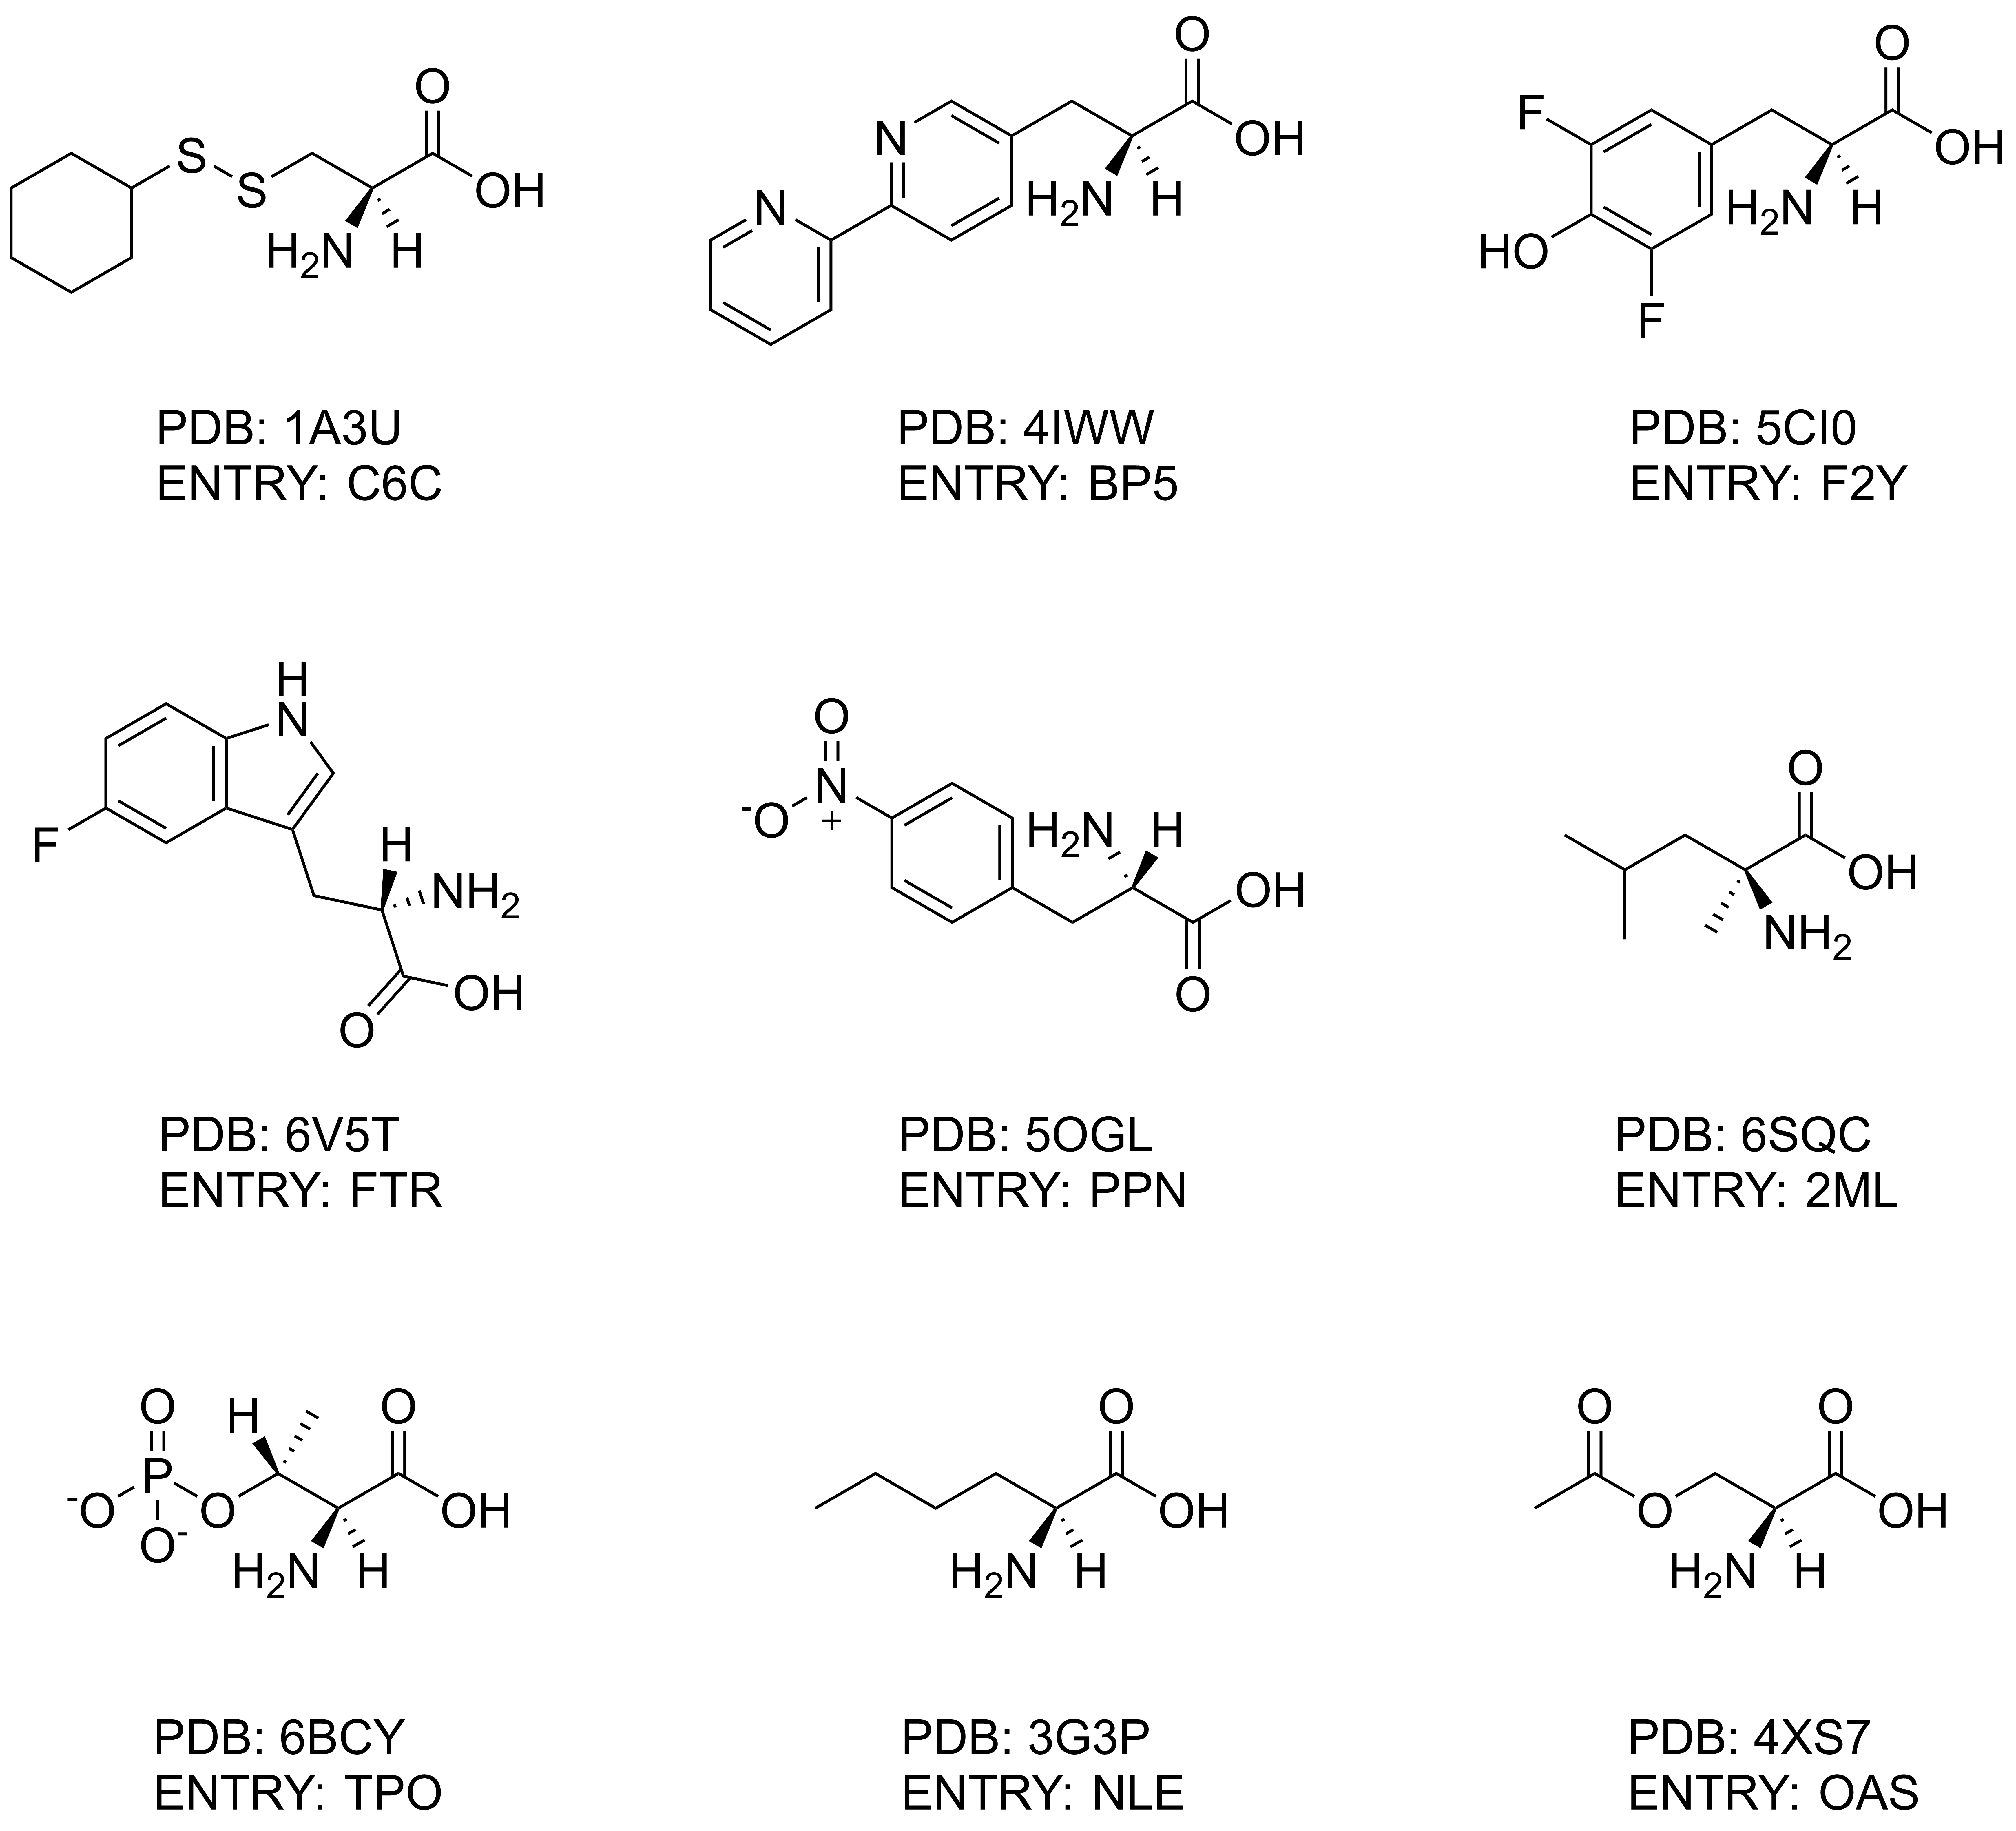
\includegraphics[width=1.0\linewidth]{benchmark.pdf}
  \caption{测试基准的选取}
  \label{fig:benchmark}
\end{figure}



\section{蛋白质文件的导入与位点突变}

为将含有非天然氨基酸的蛋白质pdb文件导入Rosetta,需要将pdb文件中非天然氨基酸各个原子的原子名称修改成与params文件中各个原子对应的原子名称。
我们采用RDKit化学工具包中子结构比对的方法完成修改。
随后,我们在RosettaScripts[29]中通过调用MutateResidue实现了蛋白质指定位点上的非天然氨基酸突变。
这一步目的是抹除蛋白质晶体结构中原有的非天然氨基酸侧链的坐标信息,以模拟非天然氨基酸侧链排布未知的情形。
需要注意的是,对于正亮氨酸NLE(对应蛋白质PDB:3G3P),由于突变位点恰好位于肽段的N端,
突变后需要在RosettaScripts中调用ModifyVariantType以补全N端的氢原子,使N端氨基带有一个单位的正电荷。



\section{结构优化}

\subsection{优化策略}
为使突变后的蛋白质重新寻找到非天然氨基酸的侧链排布状态,需要对蛋白质进行结构优化。
以ref2015为打分函数[30]进行结构优化,过程分为两步。
第一步,对蛋白质进行限制性优化:为蛋白质骨架和侧链添加坐标限制势,对蛋白质整体做放松(relax)处理。
在Rosetta的物理建模中,限制性优化可以在基本不改变蛋白质晶体结构的同时,消除原子之间不合理的冲突(比如原子间因距离较近而导致相互作用势能急剧上升)。
第一步输出50个结构,取能量最小的结构作为下一步的初始结构。
如无特别说明,我们将该结构视为后续比较分析中的“天然结构”。
第二步,对包含非天然氨基酸的局部进行结构优化:
以非天然氨基酸为中心,选择半径为\SI{12}{Å}的球壳,在内坐标空间下,打开蛋白质或多肽的骨架自由度,对球壳内的氨基酸进行侧链重排。
第二步输出1000个蛋白质结构,对此1000个结构进行数据分析。
其一,分析非天然氨基酸的构象恢复比例(rotamer recovery),即比较优化后的蛋白质中非天然氨基酸各个侧链旋转角(chi)与天然蛋白结构中各个侧链旋转角的偏差。
我们选取界限\SI{20}{°},即当旋转角差值小于\SI{20}{°}认为与天然状态相近,采样是成功的。
这一数值能够反映在当前优化策略下有多大概率能采样成功。
其二,分析在同一优化策略下,天然结构(200个结构,作为对照)与突变结构给出的score-RMSD图。
score即Rosetta对体系的打分值,反映该体系某一状态下的能量,score的值越低,该结构在Rosetta的评价体系中越稳定;
RMSD即均方根误差(root mean square deviation),类似三维坐标的RMSD计算,此处我们计算非天然氨基酸侧链旋转角的RMSD,也即
\begin{equation}
  RMSD = \sqrt{\frac{1}{n}\sum_{i=1}^n(\chi_i - \chi_0)^2}
\end{equation}
其中,
$n$表示params文件中定义的侧链旋转角的个数,
$\chi_i$表示第$i$个侧链旋转角的大小,
$\chi_0$表示天然蛋白晶体结构里非天然氨基酸中对应的侧链旋转角大小。
计算侧链旋转角的RMSD,其优点在于能够更加直观地反映侧链采样的准确率。
score-RMSD图能够反映在采样过程中,随着RMSD的减小,打分值能否随之降低进而收敛至天然构象上[31]。
需要指出的是,这里我们并不计算整个蛋白所有重原子(不包括氢原子在内的其它原子)的RMSD,而只计算单个非天然氨基酸侧链旋转角的RMSD。
如果单个非天然氨基酸侧链旋转角能够收敛,那么可以认为Rosetta能够较好地实现对该天然氨基酸的建模。
此处我们假定:当非天然氨基酸侧链采样成功时,非天然氨基酸所处的局部环境(周围其它残基的侧链排布)也能够基本模拟正确。
其三,分析打分值在前1\%(即打分最低的1\%)的蛋白结构中非天然氨基酸的侧链采样情况,即判断这些结构能成功采样前多少个侧链旋转角。
这一数据大致反映我们是否有把握以打分最低的结构代表天然结构。

按照以上优化策略和分析方法,对于选取的九种非天然氨基酸进行测试。
其中,对于磷酸化修饰的苏氨酸TPO(对应蛋白质PDB:6BCY),我们仍以第一步优化前的结构作为天然结构。
如图~\ref{fig:TPO}所示,经过第一步限制性优化后,TPO的侧链结构发生较大变化。
并且,在此例的RMSD计算中,我们不考虑第三个侧链旋转角。
这是由于在params文件定义的第三个侧链旋转角中,包含磷酸根中带负电的氧原子;
而无论是从化学性质上还是从空间位置上,末端的三个氧原子都是不可区分的。
\begin{figure}
  \centering
  \subcaptionbox{限制性优化前TPO的局部结构\label{fig:TPO_native}}
    {\includegraphics[width=0.4\linewidth]{TPO_native.png}}
  \subcaptionbox{限制性优化后TPO的局部结构\label{fig:TPO_opt}}
    {\includegraphics[width=0.4\linewidth]{TPO_opt.png}}
  \caption{限制性优化前后TPO的局部结构}
  \label{fig:TPO}
  \begin{threeparttable}
    \begin{tablenotes}
      \item [①] 以上两图中,黄色虚线表示TPO磷酸根基团中的氧原子与周围残基侧链可能形成的氢键。
    \end{tablenotes}
  \end{threeparttable}
\end{figure}

\subsection{优化结果}

对于生成的1000个蛋白结构,从采样成功率上分析,得到表~\ref{tab:sample}。
\begin{table}
  \centering
  \begin{threeparttable}[c]
    \caption{非天然氨基酸侧链旋转角的采样结果}
    \label{tab:sample}
    \begin{tabular}{ccc}
      \toprule
      非天然氨基酸   & 侧链旋转角个数    &  采样结果\tnote{①} \\
      \midrule
      C6C           &  4               &    0/0/0/0         \\
      BP5           &  3               &    1000/872/181    \\
      F2Y           &  2               &    1000/764        \\
      NLE           &  3               &    1000/1000/1000  \\
      TPO\tnote{②}  &  3               &    5/1             \\
      FTR           &  2               &    1000/1000       \\
      OAS           &  3               &    1000/1000/1000  \\
      PPN           &  3               &    1000/1000/1000  \\
      2ML           &  2               &    1000/0          \\
      \bottomrule
    \end{tabular}
    \begin{tablenotes}
      \item [①] 采样结果为p/q/r表示:在1000个结构中,成功采样前一个侧链旋转角的有p个;成功采样前两个侧链旋转角的有q个;前三个侧链旋转角的有r个。以此类推。
      \item [②] 根据前文分析,对于TPO只统计前两个侧链旋转角。
    \end{tablenotes}
  \end{threeparttable}
\end{table}
对于每一种非天然氨基酸,绘制其score-RMSD图,并比较打分最低者的结构与天然结构中非天然氨基酸的局部环境,如图~\ref{fig:score_rmsd}。
\begin{figure}
  \centering
  \includegraphics[width=1.0\linewidth]{score_rmsd.pdf}
  \caption{各个非天然氨基酸对应的score-RMSD图及局部结构}
  \label{fig:score_rmsd}
  \begin{threeparttable}
    \begin{tablenotes}
      \item [①] 对于score-RMSD图,红色点表示天然结构不经过突变直接优化得到的结果;黑色点表示经过突变后优化得到的结果。
      \item [②] 取突变后优化的结果中打分最低者(在score-RMSD图中以紫色点表示),绘制非天然氨基酸周围的局部结构图,其中绿色代表天然结构,灰色代表突变后优化的结构。
    \end{tablenotes}
  \end{threeparttable}
\end{figure}
各个非天然氨基酸中,打分值在前1\%结构中非天然氨基酸侧链的采样情况如图~\ref{fig:hits}。
\begin{figure}
  \centering
  \includegraphics[width=1.0\linewidth]{hits.pdf}
  \caption{打分值前1\%对应结构中非天然氨基酸侧链的采样情况}
  \label{fig:hits}
\end{figure}

对于含有芳香性基团(如吡啶环、苯环、吲哚环等)的非天然氨基酸,如BP5、F2Y、FTR、PPN,
以及对于具有较长侧链的NLE、OAS,基本能够正确采样所有侧链旋转角。
这些基团体积较大,能与周围残基形成较多有利的相互作用,因而更容易被正确采样。

对于C6C,比较突变后优化的结构和不经突变直接优化的结构,发现在天然蛋白结构中,C6C侧链的六元环为直立键取代,而非平伏键取代。
尽管单取代环己烷的优势构象为平伏键取代,但是在本例中,受周围残基的力场影响,C6C侧链的六元环克服与自身残基其它原子的空间位阻,选择直立键取代的构象。
值得一提的是,通过周围环境约束分子构象的例子在蛋白质设计中并不少见。
除前文提到的Mills等人捕获联苯过渡构象的例子,
Dou等人也根据类似的思路设计了β-桶状蛋白,它能将DFHBI小分子发色团约束为平面构象,从而激发荧光。

内坐标下的侧链采样并不能改变六元环的取代构象,因此我们重新绘制了直立键取代六元环的C6C分子,并给出相应的params文件进行测试,如图~\ref{fig:C6C}。
结果均能成功采样第一个侧链旋转角,其中绝大部分收敛至接近天然构象(923个结构成功采样前四个侧链旋转角),小部分收敛至另一构象(77个结构成功采样第一个侧链旋转角);
后者的打分最低值介于对照组和前者之间。
这一定程度上说明Rosetta能够从打分上挑选出天然构象。
尽管如此,可能由于突变后非天然氨基酸侧链原子的相对位置略有差异,且当前优化策略下Rosetta并不能给出更加精细的、原子级别的采样,
在只依据打分值的情况下,我们无法获得正确的结果。
\begin{figure}
  \centering
  \subcaptionbox{score-RMSD图及两种不同的构象\label{fig:C6C_score_rmsd}}
    {\includegraphics[width=0.9\linewidth]{C6C_score_rmsd.png}}
  \subcaptionbox{打分值前1\%对应结构中侧链的采样情况\label{fig:C6C_hits}}
    {\includegraphics[width=0.38\linewidth]{C6C_hits.pdf}}
  \caption{直立键取代六元环的C6C分子的采样结果}
  \label{fig:C6C}
\end{figure}


对于TPO,尽管采样成功率较低(1000个结果中只有1个正确采样前两个侧链旋转角),但采样结果收敛至天然构象,Rosetta能够对该非天然氨基酸正确建模。
如图~\ref{fig:TPO_native}所示,在天然结构中,磷酸根基团可能与周围多个残基侧链的氨基或羟基形成氢键。
这种有方向性的相互作用可能因为侧链旋转角的扰动遭到破坏,最终导致所有氨基的朝向难以同时复原,因此采样成功率较低。

对于2ML,从score-RMSD来看,尽管对照组和突变组的采样均收敛至同一构象,但均与天然结构相差较远。
结构比较显示:第二个侧链旋转角对应的旋转异构体朝向完全相反,并且骨架移动幅度较大。
与一般的结构不同,2ML对应的非天然氨基酸中α-氢被甲基取代;Rosetta对这类氨基酸可能建模较差,在后续的突变中暂不考虑。

总体而言,在蛋白质骨架与天然状态相差不大的情形下,Rosetta基本能够正确采样非天然氨基酸的第一个侧链旋转角。
